\documentclass[12pt]{article}
\usepackage{hyperref}
\usepackage[utf8]{inputenc}
\usepackage{indentfirst}
\usepackage[margin=1in, footskip=0.25in]{geometry}
\usepackage{graphicx}
\usepackage{listings}
\usepackage{makecell}
\usepackage{float}

\title{How People are Talking About the Olympic Sports}
\author{Troy Jennings\\Carl Ausmees\\Corey Vorsanger\\  \\COMP 4447: DS Tools 1}
\date{August 21, 2021}
\graphicspath{{../Images/}}
\lstset{
numbers=left, 
numberstyle=\small, 
numbersep=8pt, 
frame = single, 
language=Python, 
framexleftmargin=15pt,
framexrightmargin=15pt}

\begin{document}
    \begin{titlepage}
        {\center\huge\bfseries How People are Talking About the Olympic Sports \par}
        \vspace{1.5cm}
        \begin{center}
            Troy Jennings\\
            Carl Ausmees\\
            Corey Vorsanger\\
            \medskip
            COMP 4447: DS Tools 1\\
            \bigskip
            August 21, 2021
        \end{center}
        \begin{figure}[H]
            \centering
            
\includegraphics[scale=0.5]{tokyo.jpg}
        \end{figure}
        \begin{center}
            \textit{For a more interactive report experience please go to\\
            \href{https://github.com/cvorsanger/COMP-4447-Final-Project}{https://github.com/cvorsanger/COMP-4447-Final-Project}\\
            and launch the binder link}
        \end{center}
    \end{titlepage}

    \tableofcontents

    \section{Introduction}
        \subsection{Research Question}
            Every four years (five years sometimes) something special happens. No, it is not the world's greatest athletes coming together to showcase elite human athletisism in the Summer 
            Olympics. Rather, it is the millions of people that come together to tweet about these athletes. In a showcase of exceptional human thumbs, these people tell you all you need to know
            about the Olympics; with 100\% accuracy of course.\\ 

            So what does the twitter-sphere have to say about the Olympics? Are there sports that are being talked about in a better light then others? How does the sentiment of the Olympics 
            change over the course of the event? In this project we will be investigating tweet sentiment involving Olympic sports to see how they evolve over time. In the end the sentiment of 
            specfic sports will be analyzed and any trends should be discovered.

            \begin{figure}[htp]
                
\includegraphics[width=3in, height=2in]{Rings2.jpg}
                \hspace{0.25in}
                
\includegraphics[width=3in, height=3in]{Twitter.jpg}
            \end{figure}

        \subsection{Literature Review}
            Text sentiment analysis is really nothing new. With the advancements of Natuaral Languauge Processing (NLP) techniques building a sentiment analysis tool as become common place in a 
            wide variety of applications. While sentiment analysis is not limited to Twitter and can be used for any text data, with its vast amount of text data and constant addition of data 
            Twitter has been used in many sentiment analysis applications. From using Twitter data to help predict stock data as in 
            \href{http://cs229.stanford.edu/proj2011/GoelMittal-StockMarketPredictionUsingTwitterSentimentAnalysis.pdf}{Anshul Mittal} to the always civil discussions about politics as shown in 
            the \href{https://www.geeksforgeeks.org/twitter-sentiment-analysis-using-python/}{Geeks for Geeks article} and 
            \href{https://ieeexplore.ieee.org/abstract/document/6581022?casa_token=qrfkpDZP30sAAAAA:PNpsFf2_T9jXUB81SKLMldZji2tDprsCz4Ec4QSrHxlJQNIW3Yi52tWHZ4jhfTgPrqRjzjdKBfA}{TSAM}. 
            Unsurprisingly, there has been work done in the Olympic domain. The closest work we have discovered documented in a paper was in 
            \href{https://raw.githubusercontent.com/cvorsanger/COMP-4447-Final-Project/master/Literature%20Review/JACET_Volume%205_Issue%203_Page%20143-160.pdf}{2016 Olympic Games on Twitter: Sentiment Analysis of Sports Fans Tweets using Big Data Framework}.
            This paper came out of the Ilamic Azad University in Iran. The writter focus on Iranian Olympians instead of sports. Using tweets in both English and Farsi they classify tweets as 
            fearful, angry, surprising, sadness, joyful, neatruel, and anticipation. We will be only concerend about classifying tweets as negative, positive, or neutral.\\

            While most work follows the same general outline there are differences in sentiement analysis works. For instance 
            \href{https://raw.githubusercontent.com/cvorsanger/COMP-4447-Final-Project/master/Literature%20Review/JACET_Volume%205_Issue%203_Page%20143-160.pdf}{2016 Olympic Games on Twitter: Sentiment Analysis of Sports Fans Tweets using Big Data Framework}
            uses the WordNet package to handle most of their preprocessing and sentiment analysis model. 
            \href{https://www.geeksforgeeks.org/twitter-sentiment-analysis-using-python/}{Geeks for Geeks article} uses the TextBlob library for their sentiment analysis. 
            \href{https://towardsdatascience.com/step-by-step-twitter-sentiment-analysis-in-python-d6f650ade58d}{Yalin Yener} introduces the Vader sentiment engine in the nltk library.\\

            After review, we have decide to prusue using mostly the Natural Language ToolKit(NLTK) and the Textblob libraries. With these libraries we should be able to do most of the data 
            cleaning and allows us to use the Vader sentiment engine. More information on Vader will be presented in the Model Creation section.

    \section{Ingestion}
        \subsection{Motivation}
            A particular interest of the authors are the ongoing Summer Olympic games. We enjoy watching the top athletes in the world compete in sports that are not on television very 
            often; sports like, gymnastics,swimming, and track. A natural curioisty than was to see how other people view the Olympics.As social media has grown Twitter has been the go to 
            platform for the world to express their views. Twitter allows for people to express their feelings on just about any subject they desire (for better or for worst). It would make 
            sence then to look at Twitter data to model the sentiment around the Olympics. Luckily, Twitter provides an API  for us to query historical tweet data.

        \subsection{Ingestion}
            The twitter API is a relative easy to use API. There are a few restictions such as rate limits and API types that you do have to consider. For the purposes of this study, 
            the API makes it easy to look at historical tweets containing specific words and hashtags. The follow details certain aspects of the Twitter API that pertains to this 
            project. For more information please visit \href{https://developer.twitter.com/en/docs/twitter-api}{here}. \\

            The first step is to get authorization. To get this we must provide the API with our given client key and secret using the POST command with the requests library. Once we get
            POST we will recieve a response from the API we must save.
            
            \begin{lstlisting}[caption=Authorization]
import numpy as np
import pandas as pd
import requests 
import base64

# Save Authorization Info.
client_key = 'XXXXXXXXXXXXXXXXXXXXXXXXXX' 
client_secret = 'XXXXXXXXXXXXXXXXXXXXXXXXXX' 
bearer_token = 'XXXXXXXXXXXXXXXXXXXXXXXXXX' 
key_secret = '{}:{}'.format(client_key, client_secret) \\
    .encode('ascii')
b64_encoded_key = base64.b64encode(key_secret)
b64_encoded_key = b64_encoded_key.decode('ascii')

# Build API URL 
base_url = 'https://api.twitter.com/'
auth_endpoint = base_url + 'oauth2/token'
auth_headers = { 'Authorization': 'Basic {}'  \\
    .format(b64_encoded_key),
                'Content-Type': \\
    'application/x-www-form-urlencoded;charset=UTF-8' }
auth_data = { 'grant_type': 'client_credentials' }

# Provide Authorization Info and Save Access Token
response = requests.post(auth_endpoint, headers=auth_headers, \\
    data=auth_data)
print("Response Status Code: ",response.status_code)
            \end{lstlisting}

            As expected we get a response status code of "200". This tells us that we succesfully recieved our response. The next step is to get the \textit{access token} from our 
            authorization response. \\

            A utility function was then created. This function allows us to use the twitter API to save tweets. The function needs the users saved access token and allows for the user 
            to specify the number of tweest to pull. The most important parameter of this function is the query parameter. This allows for you filter the tweets you recieve by specific 
            hashtags, words, retweets, etc. For this project we are concerned with tweets containg the hashtags "\#olympics" and containing the a specific sport.

            \begin{lstlisting}[caption=Tweet Generator]
def get_tweets(access_token, query, max_tweets=10, tweet_limit=10):

    page_token = None
    tweet_data = []
    search_headers = {
        'Authorization': 'Bearer {}'.format(access_token),
        'User-Agent': 'v2FullArchiveSearchPython',
    }
    # Divides the max tweets into the appropriate number of 
    # requests based on the tweet_limit.
    for i in range(max_tweets // tweet_limit - 1):
        search_parameters = {
            'query': query,
            'max_results': tweet_limit,
            'tweet.fields': 'lang,created_at,referenced_tweets, \\
                source,conversation_id'
        }
        # If we reach the 2nd page of results, add a next_token 
        #attribute to the search parameters
        if i > 0:
            search_parameters['next_token'] = page_token

        response = requests.get(search_url, headers=search_headers,\\
            params=search_parameters)
        if response.status_code != 200:
            print(f'\tError occurred: Status Code{response. \\
                status_code}: {response.text}')
        else:
            # We need to check for a result count before doing 
            # anything futher; if we have result_count we have data
            if response.json()['meta']['result_count'] > 0:
                tweet_data.extend(response.json()['data'])
                
                # If a 'next_token' exists, then update the page 
                # token to continue pagination through results
                if 'next_token' in response.json()['meta']:
                    page_token = response.json()['meta']['next_token']
            else:
                print(f'\tNo data returned for query!')
                break        
        print(f'\t{len(tweet_data)} total tweets gathered')
        time.sleep(1)
    return tweet_data
            \end{lstlisting}

            Using the above function we can sample retweets having to do with olympic gymnastics. Notice that we are specify the hashtag "\#olympics", the word "gymnastics" and is a 
            retweet in the query parameter. Finally, so we do have to keep requesting data from the twitter API we save the tweets in a pickle file. This way we can use them later in 
            our anaysis (and twitter will not get mad at us for rate limits).\\
            
            Using the \textit{get\_tweets} function we tried to pull 5000 tweets for the sports basketball, biking, diving, gymnastics, skateboarding, surfing, track, and volleyball. This was 
            easily done by changing the query parameter to include the name of the sport.

        \subsection{Sample and Explanation}
        Alright we have pulled in some tweets. Now lets have a look at some of the original tweets and the retweets.
        \begin{center}
            \begin{tabular}{ |c|c|c|c| }
                \hline
                text snippet & id & created\_at & conversation\_id \\  
                \hline
                \makecell{c\@Shawn\_Shipp\_ Thank You, \\ Simone Biles - Headph...} & 1423371158443941890 & \makecell{2021-08-05 \\ T19:51:43.000Z} & 1423299151215931392 \\
                \hline
                \makecell{Unexpected fun fact: \\ Liu Yang originally wa...} & 1423471713312854017 & \makecell{2021-08-06 \\ T02:31:17.000Z} & 1423471713312854017 \\
                \hline
                \makecell{Rhythmic Gymnastics looks \\ insane. \#Olympics} & 1424213988720717828 & \makecell{2021-08-08 \\ T03:40:50.000Z} & 1424213988720717828 \\
                \hline
                \makecell{\@kpkuehler Thank You, \\ Simone Biles - Headphone...} & 1423796825761456128 & \makecell{2021-08-07 \\ T00:03:10.000Z} & 1423616706413572103 \\
                \hline
                \makecell{\@Simone\_Biles you are \\ a wonderful human being ...} & 1423812938889142273 & \makecell{2021-08-07 \\ T01:07:12.000Z} & 1423812938889142273 \\
                \hline
            \end{tabular}
        \end{center}
        There is a lot of information about tweets that you recieve can recieve from the API. We have narrowed it down to the important ones for this study:
        \begin{itemize}
            \item text - The text of the tweet sent out. This will include user handles, hastags, emojis, and any retweet indicators
            \item id - The unique id given to the tweet. This allows for twitter to store tweets.
            \item created\_at - When the tweet was tweeted. Given in UTC time.
            \item conversation\_id - The unique id given to twitter conversations. We can use this id to get all tweets in an conversation.
        \end{itemize}
    \section{Data Cleaning}
        \subsection{Initial Exploration and Cleaning}
            So, now we have tweets regarding the olympic sports of basketball, biking, diving, gymnastics, skateboarding, surfing, track, and volleyball. All of the tweets were collected
            into a single dataframe. This will make it easier for us to clean, look at, and use all of the tweets at once. During this process a new variable was created,
            \textit{sport}. This varibale will track for us the sport that each tweet is talking about and allows us to segment the tweets later when we build our sentiment model. \\
        
            Using the shape function we find that we have 30554 tweets. Now, time to get our hands dirty and clean the data. \\
        
            As with all text data there is alot of cleaning that can be done. For this project we will be concentrating on removal of certain entities such as url links and hashtags, removal
            of stopwords, lemmatization, and general NLP text cleaning. After this NLP specific cleaning we should be ready to analyze the sentiment of tweets.\\

            Using the below function we were able to use regular expressions to filter the text of our tweets. This function will remove urls, user handles, hashtags, punctuations, new line 
            characters, and numbers that are in the text of the tweet. \\

            \begin{lstlisting}[caption=Regular Expression Cleaner]
import re
def clean_tweet_text(text):
    # Define any custom replacement pattern and join into an 
    #aggregated pattern
    replacements = [
        r'(@[\w]+)',
        r'http[s]?://(?:[a-zA-Z]|[0-9]|[$-_@.&+]|[!*\(\),]|(?:%[0-9\\ 
            a-fA-F][0-9a-fA-F]))+',
        r'(#\w+)',
        r'[\$&+,:;=?@#|\'<>.^*()%!-/]',
        r'\n',
        r'[0-9]+'
    ]
    aggregate_pattern = r'|'.join(replacements)
    # make regex substitutions in one pass
    clean_text = re.sub(aggregate_pattern, '', text) 
    
    # Return the unicode-stripped text in lowercase
    return clean_text.encode(encoding='ascii', errors='ignore')\\
        .decode('ascii').lower()
            \end{lstlisting}

            Stopwords are common words in the English language such as the, an, a, etc. These words are used much in English but convey little meaning. In most NLP applictions stop 
            words have very little value and only slow down your model due to their high frequency. In sentiment analysis they also have the potential to skew our model toward a neutral
            outcome. The NLTK library has provides a wide assortment of tools to use for NLP. It even includes a list of stopwords we can use. By iterating over our text and comparing
            the text to the list of stopwords we can remove them for our tweets. \\

            Next we will lemmatize our tweets. Lemmatization is a process where words are converted to their dictionary forms. For instance the word "walking" will be analyzed as "walk". 
            Lemmatization will ensure that we have proper words. This is the main reason why we chose to lemmatize instead of stemming as the lexicon in Vader works much better with real 
            words. The NLTK library has a function **WordNetLemmatizer** built in. We will the **WordNetLemmatizer** to handle the lemmatization for us. \\

        \subsection{Type Conversion}
            We needed to change a few data types. Thankfully, the tweet text was already given to us as an object (string). To make our analysis easier we changed the \textit{tweet id} and the 
            \textit{conversation ids} of type int from type object. To facilitate the time aspect of our analysis we needed to also covert the \textit{created\_at} variable to a datetime object.\\

            This leaves us with these variable types, the correct variable types:
            
            \begin{center}
                \begin{tabular}{|c|c|}
                    \hline
                    id & int32\\
                    \hline
                    created\_at & datetime64[ns, UTC]\\
                    \hline
                    conversation\_id & int32\\
                    \hline
                    text & object\\
                    \hline
                    sport & object\\
                    \hline
                    withheld & object\\
                    \hline
                    clean\_text & object\\
                    \hline
                    clean\_no\_stops & object\\
                    \hline
                    lemma\_text & object\\
                    \hline
                \end{tabular}
            \end{center}
        \subsection{Missing Values}
            Twitter keeps track of everything about a tweet. This is good news to us because the twitter API rarely gives you missing values. The below missing value plot shows that there is no 
            important missing values. \\

            In fact all of the missing values appear to be in the withheld column. The "withheld" column just tells us in which countries these tweets are not allowed in. This is not
            important in our analysis and we will therefore just drop that column.
            \begin{figure}[H]
                \centering
                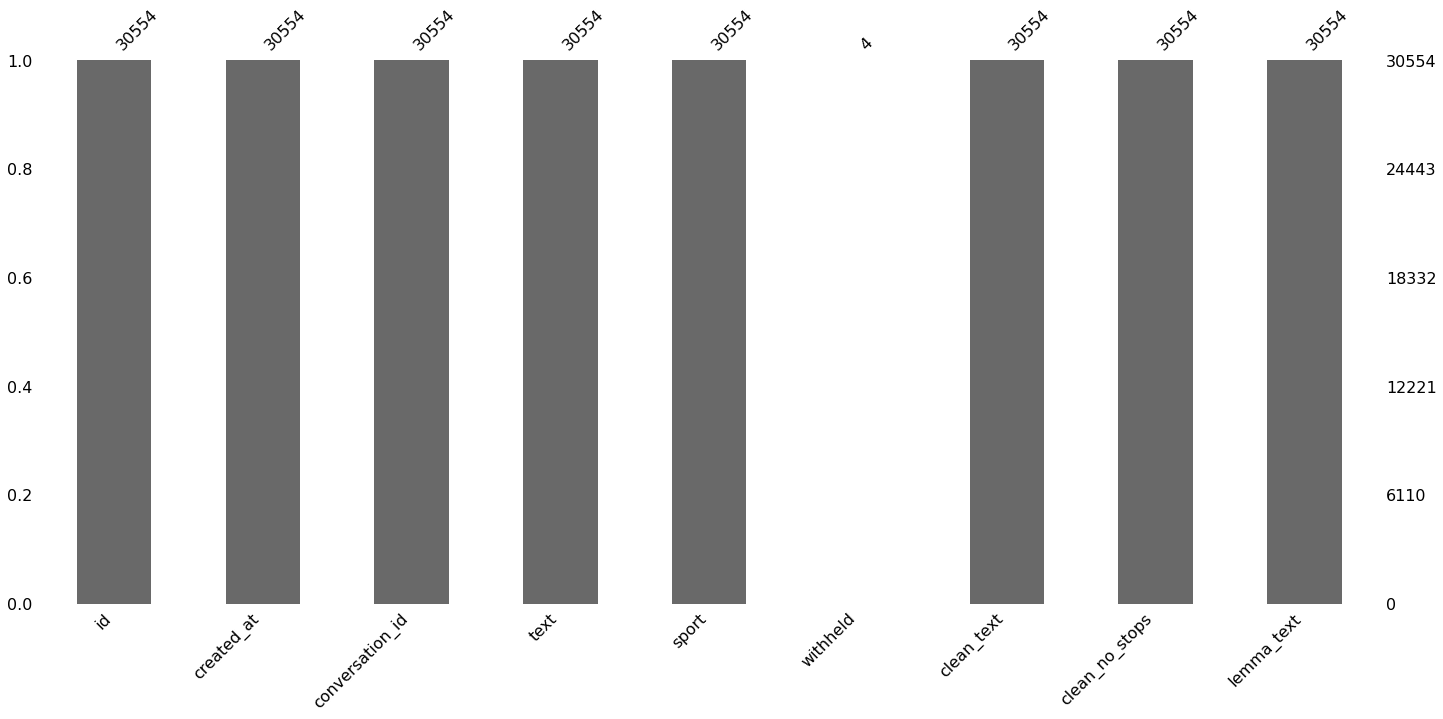
\includegraphics[scale=0.33]{missing.png}
            \end{figure}
        \subsection{Outliers}
            With text data it can be difficult to define what an outlier is. Obviously, people can say obnoxiously positive and negative stuff without really nowing anything; this 
            \textit{definatly} doesn't happen on twitter (wink wink). However, the only real way to detict this is after the sentiment model is built. Also how do we know what are 
            genuine tweets that should be factored in our anaysis and bogus tweets that should not. We do assume that most people that are tweeting about the Olympics are at least 
            watching them. This is also our main target audience in this study; average peeople watching the Olympics. With it being impossible to detect bogus tweets from the API 
            and our assumption that a vast majoroity of our tweets originate from our target audience, we decide to anaylze all of the tweets we could get. Potentially this could skew
             our sentiment scores. However, we feel confident that with the number of good tweets this potential skew effect should be drowned out.
        \subsection{Additional Exploration}
        \begin{figure}[H]
            \centering
            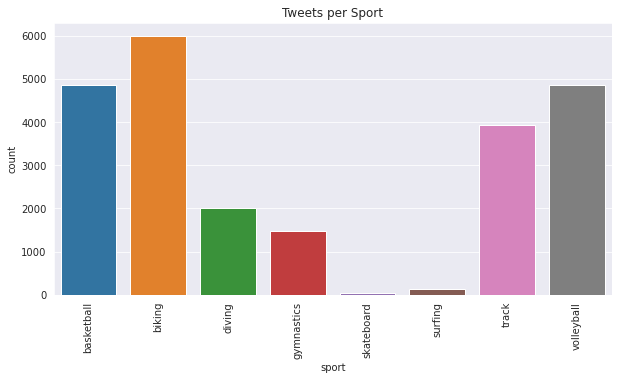
\includegraphics[scale=0.5]{sporttweet.png}
        \end{figure}
            \begin{figure}[H]
                \centering
                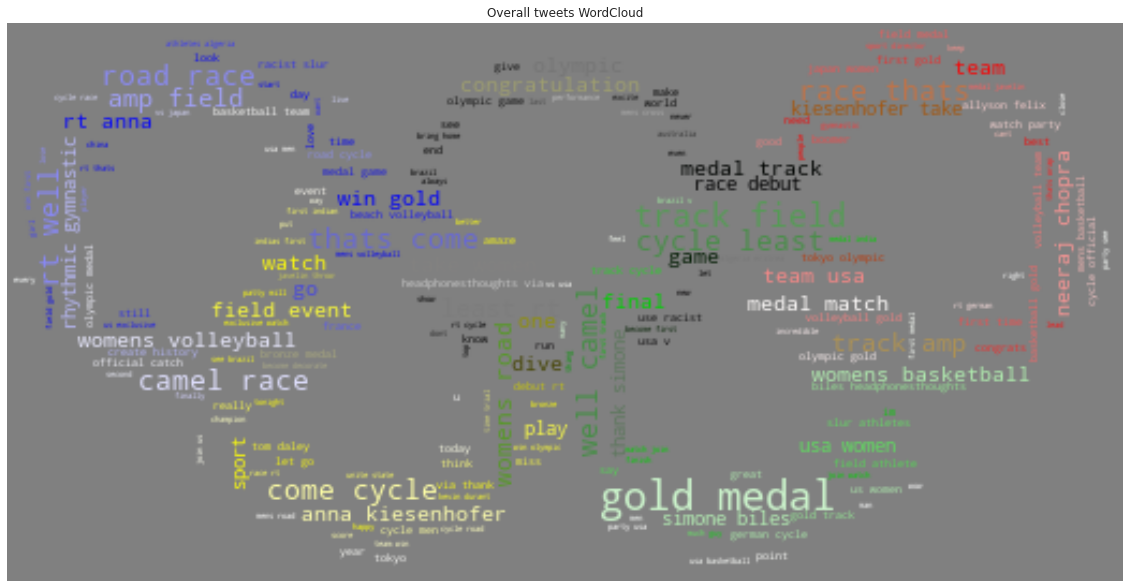
\includegraphics[scale=0.4]{wordcloud.png}
            \end{figure}
            \begin{figure}[H]
                \centering
                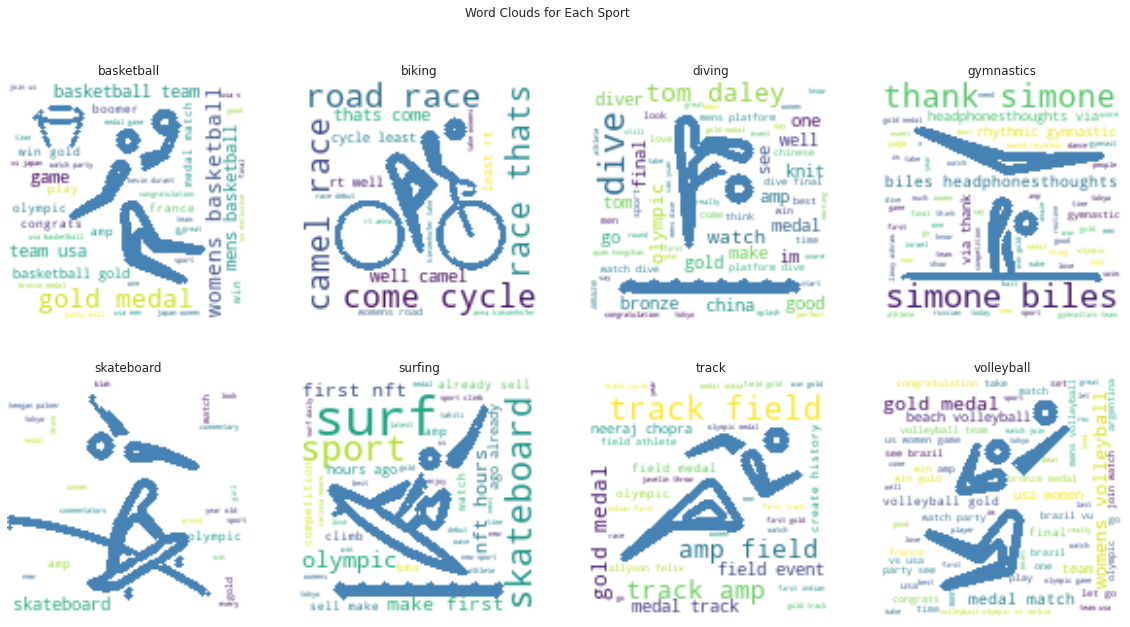
\includegraphics[scale=0.4]{sportsclouds.png}
            \end{figure}
    \section{Model Creation}
        \subsection{Model}
    \section{Evaluation and Conclusions}
        \subsection{Results}
        \subsection{Future Work}
\end{document}